\section{Approach and research methodology}\label{approach}

\subsection{Datasets}\label{datasets}
We have found two datasets which we decided to work on:
\begin{itemize}
    \item \textit{Song lyrics from 79 musical genres} dataset from Kaggle website \cite{KaggleDataset},
    \item \textit{MetroLyrics} dataset processed and put in a GitHub repository \cite{GithubDataset}.
\end{itemize}

In the description of the first dataset, we can find the information that the dataset consists of 379 893 song lyrics from 4239 artists. Around 50\% of the song lyrics are in English and we test our models on them. Information about the artists is kept in a separate file and contains a list of music genres each artist is connected with. As we predict only one music genre for each song we preprocess this dataset by reducing these lists to individual genres (we take the first one from the list) and assigning them to song lyrics of appropriate artists. Furthermore, we preprocess song lyrics as they contain punctuation and span across multiple lines.

By contrast, the second dataset required minimal work on our site. It was initially published on Kaggle website and consisted of 362 237 song lyrics from 18231 artists. The majority of song lyrics (probably around 60\%) were in English. Unfortunately, this dataset was removed from Kaggle website and we were not able to find it in its original form anywhere else. We have found a preprocessed version of it in a GitHub repository of a students' project performed by University of California students in 2018. This version's song lyrics have punctuation removed and contain only one genre for each entry.

\subsection{Datasets preparation}\label{Datasets preparation}

First of all, we conducted some basic preparations of datasets.
For \textit{MetroLyrics} we decided to remove genre \textit{Other} and merge genres \textit{Country} and \textit{Folk} since  our research showed they are very similar, and additionally the second was significantly smaller in samples. As for \textit{Song lyrics from 79 musical genres}, we filtered songs to only English ones and omitted the genre \textit{Pop/Rock} since it is ambiguous.

After conducting a few simple tests on the whole dataset we decided to limit ourselves to a much smaller part of the observations. There were two main reasons for that: limited resources and time - we would not manage to conduct all desired tests on the whole dataset, and second - the dataset was very strongly unbalanced and therefore accuracy was often significantly bigger than balanced accuracy. To solve both problems we decided to limit ourselves to only five genres with the biggest number of samples: \textit{Rock}, \textit{Pop}, \textit{Metal}, \textit{Hip-hop} and \textit{Country}.

In the end, we conducted tests on two datasets:
\begin{itemize}
    \item Balanced dataset with lyrics from 5 genres, $116,120$ observations in total, created from both \textit{MetroLyrics} and \textit{Song lyrics from 79 musical genres} datasets.

    \item Unbalanced dataset with lyrics from 5 genres, $262,122$ observations in total, created from both \textit{MetroLyrics} and \textit{Song lyrics from 79 musical genres} datasets.
\end{itemize}

\subsection{Text preprocessing}

Since in our project, we use embeddings that may be or even should be used on the raw text we decided to test two approaches: one with strong and the second with weak preprocessing of text.

Weak preprocessing consists of deleting numbers in the text and some words characteristic of lyrics notation (e.g. "VERSE", "CHORUS", "2x"). We decided to also expand contractions since they were proven to be troublesome in further preprocessing such as tokenization or removing stopwords. We deleted all special characters since interpunction was used inconsistently in most songs (e.g. lyrics usually didn't have a division for sentences). We also lowered the whole text since every verse began with a capital letter which usually had nothing to do with starting a sentence. Thanks to that we could also use uncased versions of embeddings.

Strong preprocessing consists of, besides the above, tokenization, lemmatization, and deleting stop words. For these steps, we used \textit{nltk} package.



\subsection{Division into two models}

Since one of the datasets is very unbalanced (the amount of Rock genre observations is two times more numerous than all other genres together) we decided to try an approach that will classify the largest genre class separately from the rest. Therefore we prepared a 2-step CNN classifier that consists of two sub-classifiers: a BinaryCNN classifier which only recognizes if lyrics are of the one selected genre or not, and a multiclass CNN classifier (the same is used as a normal classifier for all genres) which classifies all other genres.

\begin{figure}[!h]
\centering
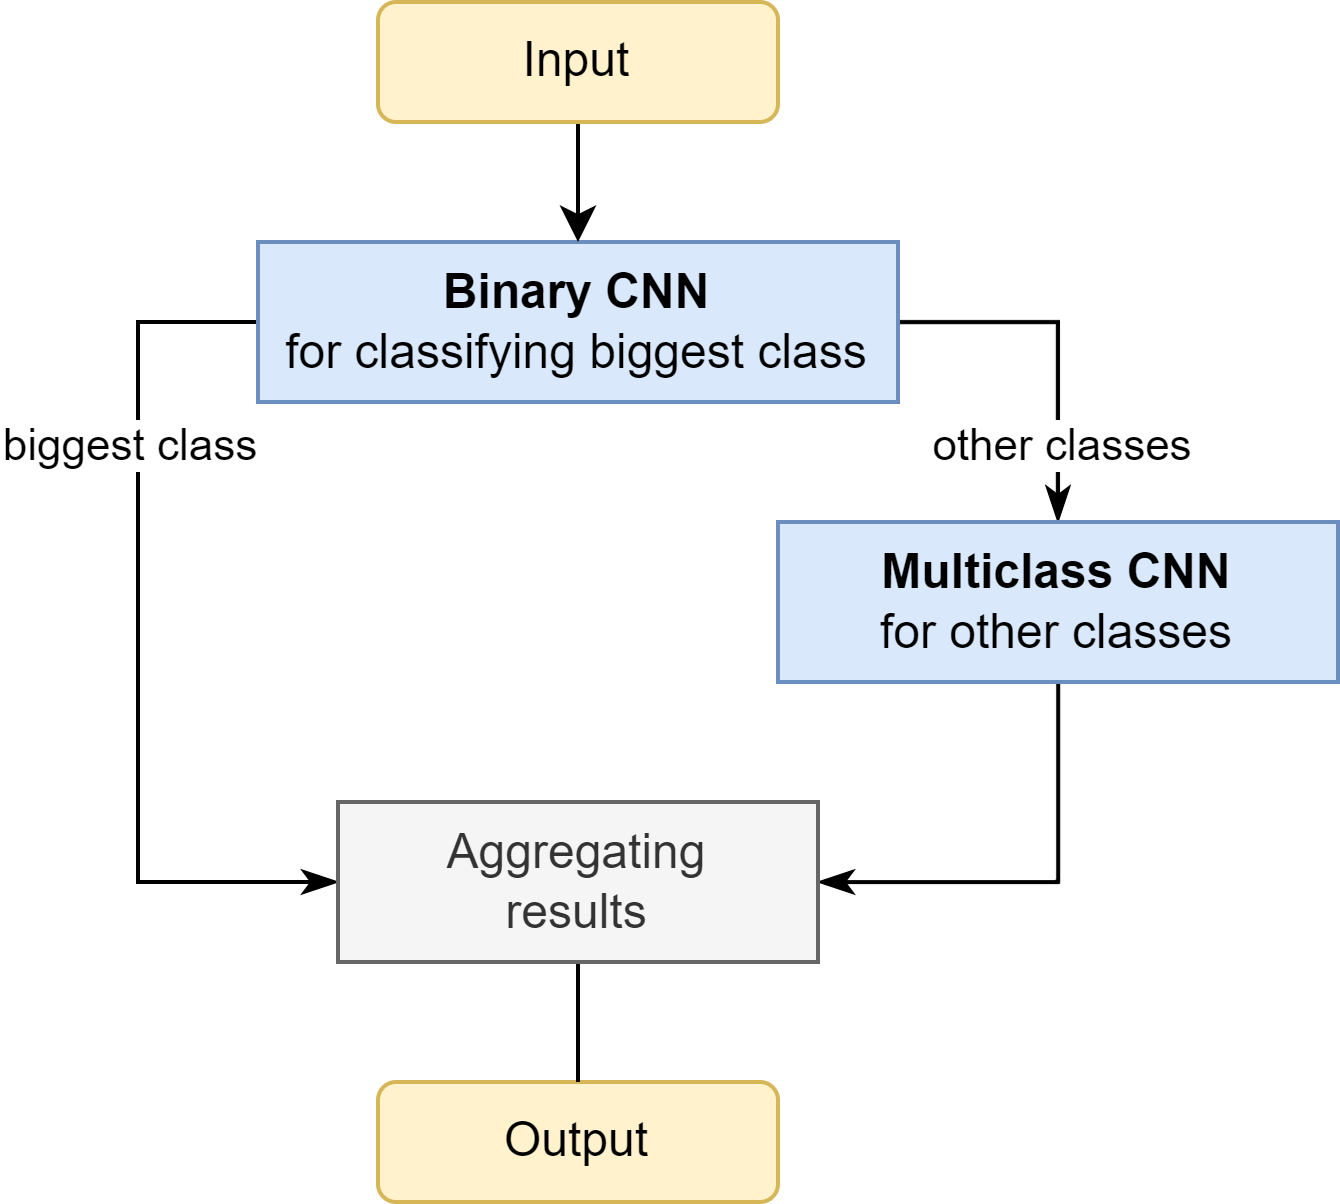
\includegraphics[width=7cm]{plots/2step_cnn_schema.drawio.png}
\caption{2-step CNN architecture}
\end{figure}

In this way, we hope to better recognize and separate the Rock genre and influence significantly balanced accuracy.


\subsection{Creation of the dataset}
We decided to create our own dataset using Spotify API \cite{Spotify} and Genius API \cite{Genius}. We wanted to use Spotify to get tracks from chosen genres and Genius to get lyrics of returned songs. At first, we utilized the \textit{Get Recommendations} endpoint. Unfortunately, the recommended songs repeated a lot between different API calls. That meant that after dropping duplicates we were left with a few times less observations than desired. To deal with this issue, we decided to use the \textit{Search for Item} endpoint. This endpoint allows specifying genre but limits the possible output to the first 1000 tracks. Another problem that we faced was that Genius did not always have the lyrics to the songs provided by Spotify. And even if it did sometimes instead of proper lyrics text of books or different lists of artists and the titles of their songs were returned. Because of that the created dataset needed also manual data cleaning. At last, in that way, we created the dataset containing 5 genres and 4,092 observations. Table \ref{tab:our_dataset_genres} presents the number of observations in each genre.

\begin{table}[h]
\centering
\begin{tabular}{l|r}
\textbf{Genre} & \textbf{Number of observations} \\\hline
country & 896 \\
metal & 887 \\
pop & 815 \\
rock & 767 \\
hip-hop & 727 \\
\end{tabular}
\caption{The number of observations in each genre in created dataset}
\label{tab:our_dataset_genres}
\end{table}
